\documentclass{acm_proc_article-sp}
\usepackage{url}

\begin{document}
\title{Demo: Spectrum Agile mm-Wave Packet Radio}
%
% You need the command \numberofauthors to handle the 'placement
% and alignment' of the authors beneath the title.
%
% For aesthetic reasons, we recommend 'three authors at a time'
% i.e. three 'name/affiliation blocks' be placed beneath the title.
%
% NOTE: You are NOT restricted in how many 'rows' of
% "name/affiliations" may appear. We just ask that you restrict
% the number of 'columns' to three.
%
% Because of the available 'opening page real-estate'
% we ask you to refrain from putting more than six authors
% (two rows with three columns) beneath the article title.
% More than six makes the first-page appear very cluttered indeed.
%
% Use the \alignauthor commands to handle the names
% and affiliations for an 'aesthetic maximum' of six authors.
% Add names, affiliations, addresses for
% the seventh etc. author(s) as the argument for the
% \additionalauthors command.
% These 'additional authors' will be output/set for you
% without further effort on your part as the last section in
% the body of your article BEFORE References or any Appendices.

\numberofauthors{1} %  in this sample file, there are a *total*
% of EIGHT authors. SIX appear on the 'first-page' (for formatting
% reasons) and the remaining two appear in the \additionalauthors section.
%
\author{
% You can go ahead and credit any number of authors here,
% e.g. one 'row of three' or two rows (consisting of one row of three
% and a second row of one, two or three).
%
% The command \alignauthor (no curly braces needed) should
% precede each author name, affiliation/snail-mail address and
% e-mail address. Additionally, tag each line of
% affiliation/address with \affaddr, and tag the
% e-mail address with \email.
%
% 1st. author
\alignauthor
Julian Arnold, Ljiljana Simi\'{c}, Marina Petrova, Petri M\"ah\"onen\\
       \affaddr{Institute for Networked Systems}\\
       \affaddr{RWTH Aachen University}\\
       \affaddr{Kackertstrasse 9, 52072 Aachen, Germany}\\
       \email{\{jua,lsi,mpe,pma\}@inets.rwth-aachen.de}
}

\date{\today}

\maketitle
\begin{abstract}
We are presenting a spectrum agile mm-Wave packet radio communication system for multimedia streaming purposes.
The proposed system operates in the 60 GHz 70 GHz and 80 GHz bands.
\end{abstract}

% A category with the (minimum) three required fields
%\category{H.4}{Information Systems Applications}{Miscellaneous}
%A category including the fourth, optional field follows...
%\category{D.2.8}{Software Engineering}{Metrics}[complexity measures, performance measures]

%\terms{Theory}

\keywords{mm-Wave, SDR, USRP, GNURadio} % NOT required for Proceedings

\section{Introduction}
The demand for high capacity connections is rapidly growing theses days driven by the increasing amount of data demanding multimedia applications. 
One promising solution to cover this demand is the uses of the mm-Wave band which provides a large amount of currently unoccupied bandwidth. 
While there are already some commercial products out there which make use of this band \cite{vubiqnetworks} \cite{hxi} there are almost no open implementations that enable and drive support for MAC and PHY layer protocol research.
To the best of our knowledge we are among the first to provide an open-source packetized radio system than can operate in several mm-Wave bands and that is highly reconfigurable due to the use of software defined radios.
In \cite{Zhu14} the authors demonstrate the feasibility of 60 GHz links for outdoor pico-cells. They also did extensive measurements. However, they were using of the shelf hardware to proof their assumptions which does not allow modifications of the lower layers.
In \cite{Zetterberg15} the authors demonstrate an open-source 60 GHz transceiver design which is also compatible to USRP software defined radios. While this is indeed a big step forward the authors were mainly focusing on the hardware design and the evaluation of it. Furthermore, the design is open hardware but it still takes some efforts to actually fabricate the transceiver if one wants to use it.
Using our system the user can easily implement and test its own PHY and MAC layer protocols and see how they behave in a real world environment.

\section{Design and Implementation}
Figure \ref{fig:block} shows a block diagram of the proposed system. 
We use a host PC running GNURadio \cite{gnuradio} to generate a complex sample-stream at baseband. The sample-stream is packetized and send to a USRP \cite{ettus} software defined radio via Ethernet.
The USRP transfers the complex baseband signal to a passband signal at an intermediate frequency between 1.2 GHz and 6 GHz. The exact intermediate frequency can easily be adjusted via the GNURadio program. Because of the wide IF range and the ability to change the frequency during runtime the system can operate very spectrum agile allowing it to avoid interference with other transmissions.
In order to transfer the signal into the mm-Wave band an external up-converter is used. It is worth mentioning that the system can be operated in the 60 GHz, 70 GHz and 80 GHz bands.
The up-converted signal is then emitted using a wave guide connected horn antenna.
On the receive side basically the same processing is applied but using a down-converter and the USRP as a receiver. The complex sample stream is fed back to the same host PC and processed in the GNURadio application where synchronisation and demodulation is applied.
Our implementation is open source and details can be found at \cite{gr-inets}. 

During the demo session we will demonstrate the proposed system, showing its operation in several mm-Wave bands.

\begin{figure}
\center
\includegraphics[width=0.4\textwidth]{block-diagram}
\caption{Block Level Description}
\label{fig:block}
\end{figure}

\begin{figure}
\center
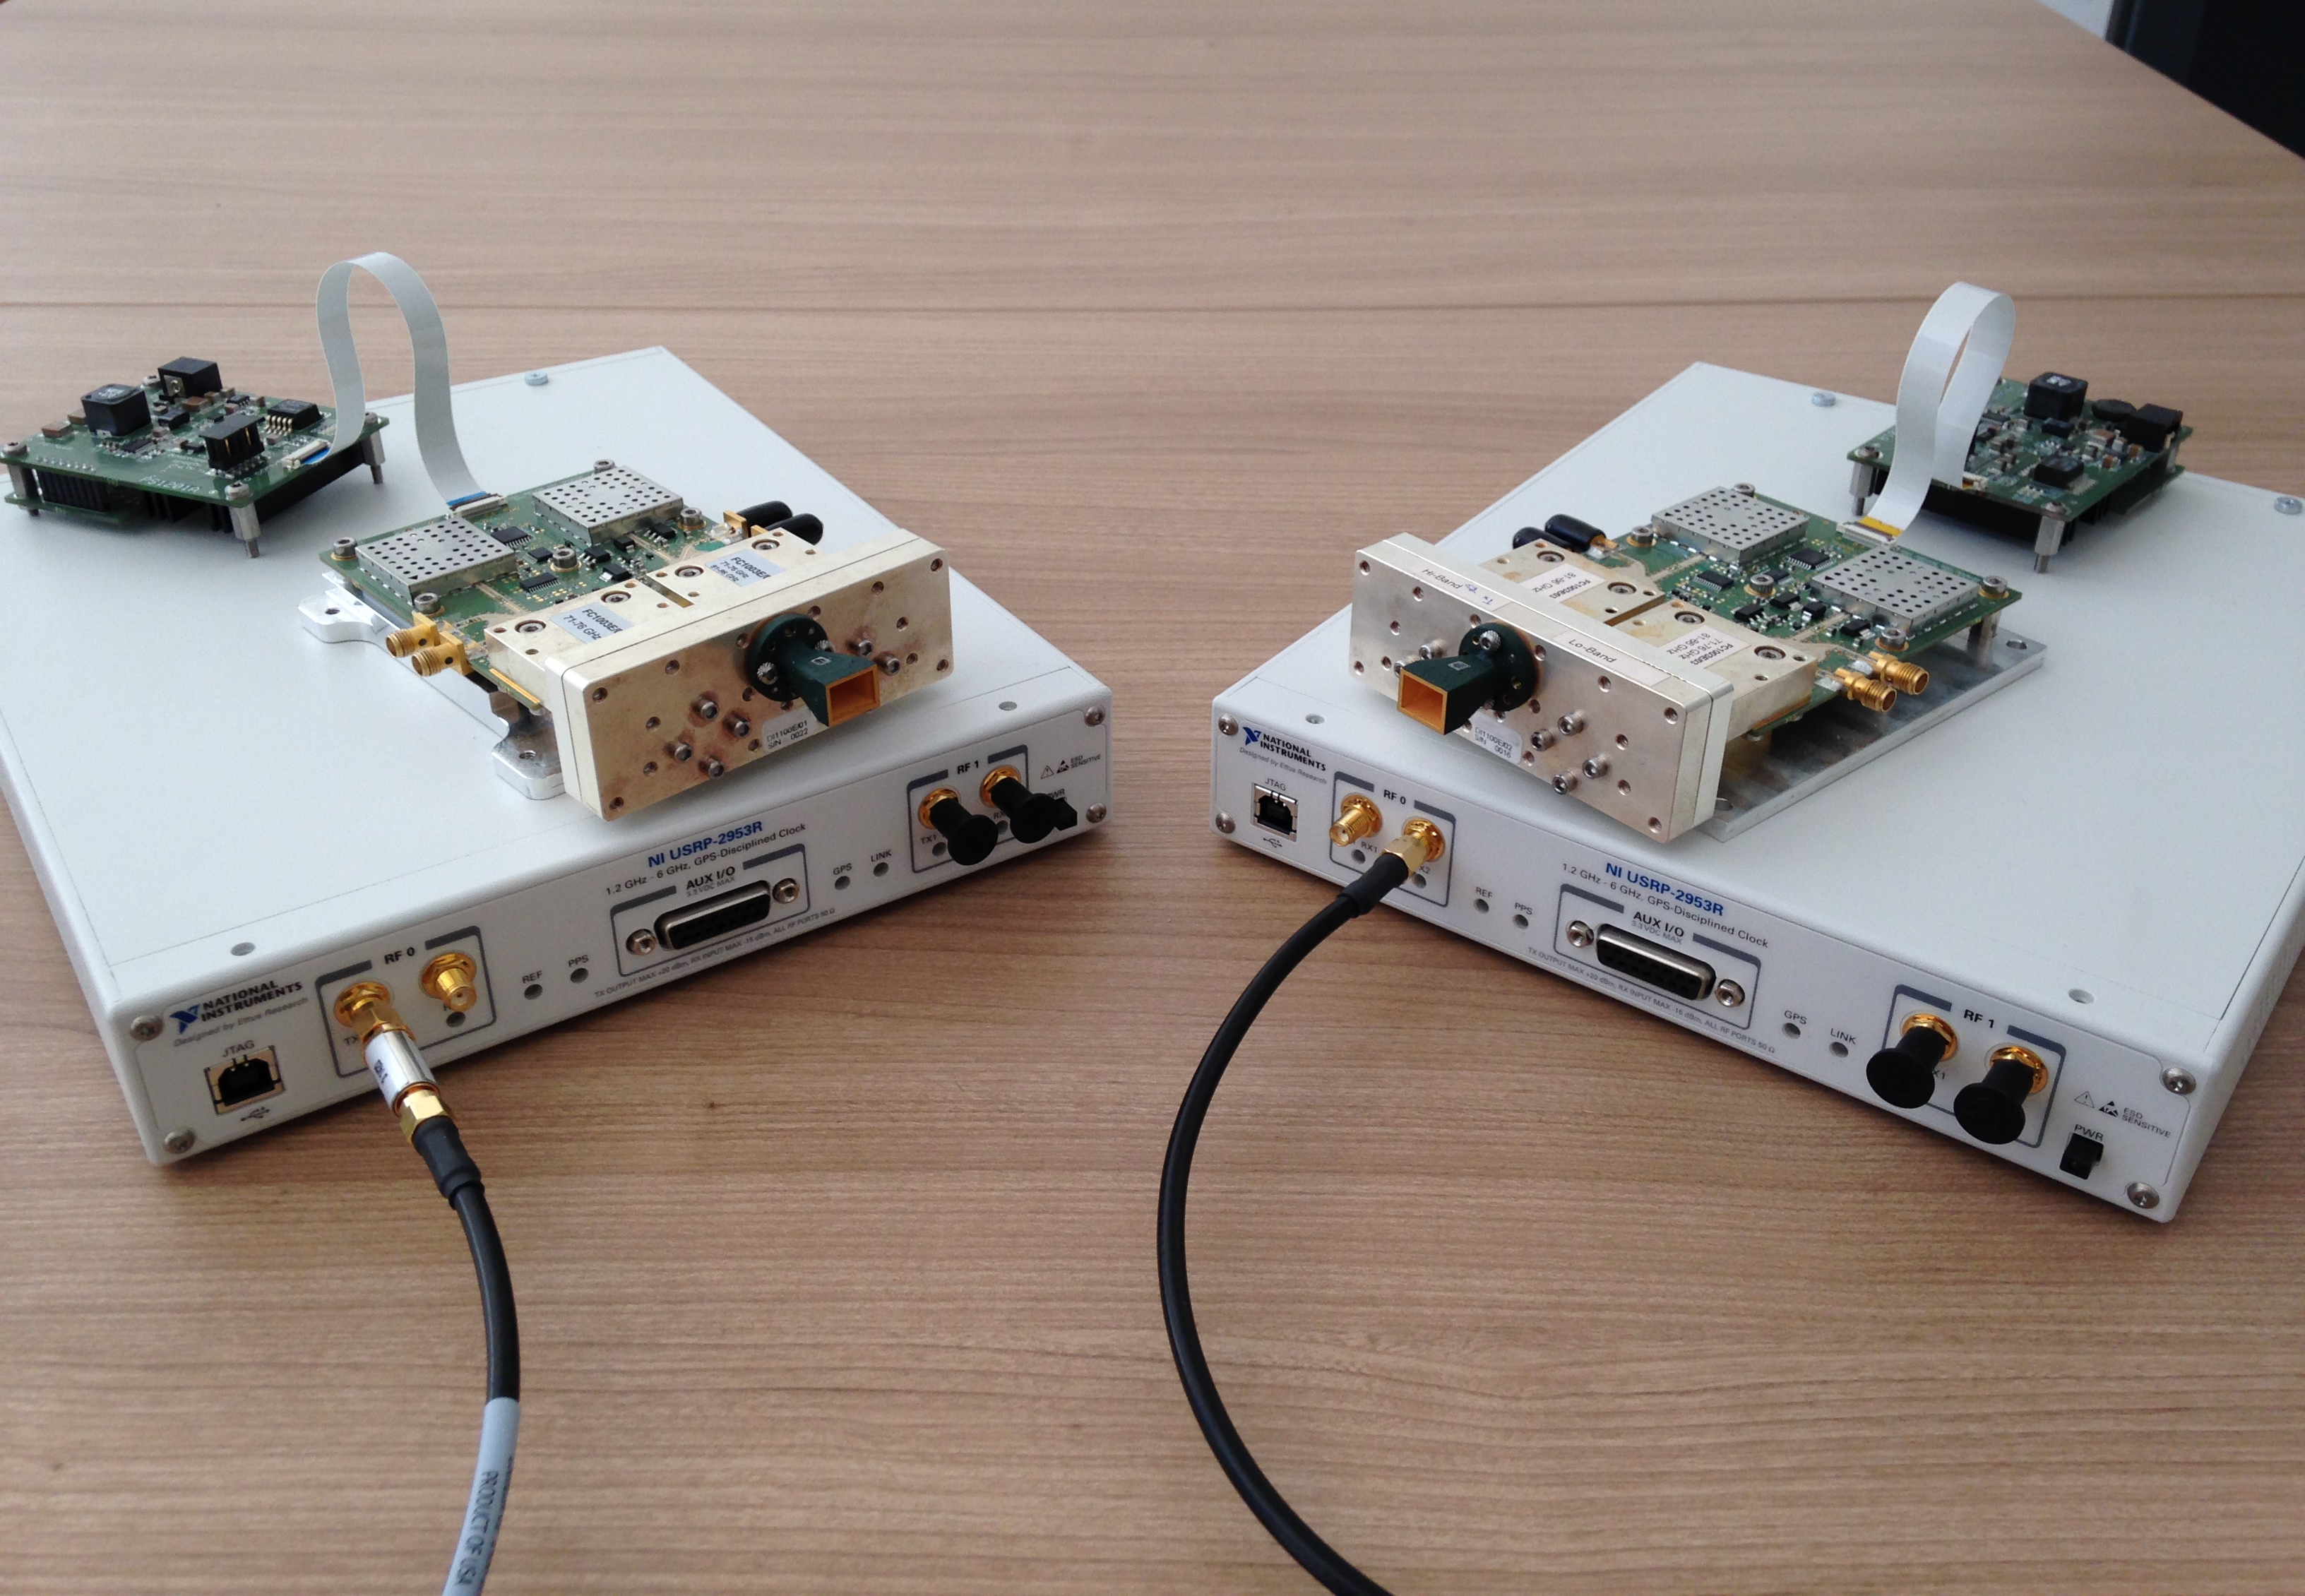
\includegraphics[width=0.4\textwidth]{system.jpg}
\caption{System Overview}
\label{fig:system}
\end{figure}
\balancecolumns
\section{Conclusion}
We demonstrated an open source mm-Wave communication system for packetized multimedia applications. Furthermore, we showed the easy reconfigurability of our system due to the use of software defined radios which will drive new MAC and PHY layer developments for the mm-Wave band.

%\begin{figure}
%\begin{tikzpicture}
%\draw[thick] (0, 0) rectangle (1,1) node[pos=.5] {USRP};
%\draw[thick, ->] (1,.5) -- (2,.5);
%\draw[thick] (2.4, 0.5) -- (3,.5);
%\end{tikzpicture}
%\caption{Do not forget!
%Make it explicit enough that readers
%can figure out what you are doing.}
%\end{figure}

\bibliographystyle{abbrv}
\bibliography{sigproc}
\balancecolumns
\end{document}